\chapter{Data-Parallel Architectures}
Data-parallel architectures are parallel over individual records of data. This can be each cell in a matrix, each pixel of an image, every record of a database, or more.

\section{Connectivity}
\label{sec:connectivity}
We want to support basic computations required at the cell level. As an example:
\[ A[i,j] = (A[i-1,j] + A[i+1,j] + A[i,j-1] + A[i,j+1])/4 \]

To achieve this, individual processing units \footnote{or cells, or nodes, or whatever your preferred terminology may be} can be connected in a variety of ways: \begin{itemize}
\item \textbf{Nearest Neighbours}: Mapping spatially-coherent data (like images) onto SIMD systems. It is common to connect to the cardinal directions, but diagonal connections have also been implemented. This has been applied to massively parallel systems, is scalable, and simple to implement.
\item \textbf{Trees and Graphs}: Problems expressed as graphs (such as database searching, model matching, expert systems, etc). These have no mathematically regular structure. As a result, the architecture will require reconfigurability. Binary and quadtrees are common. Data bottlenecks are possible when traversing the roots of subtrees.
\item \textbf{Pyramid}: The pyramid structure is a combination of a mesh and tree, depicted in \autoref{fig:screenshot096}. It supports nearest neighbour and quadtree communication; local communication is done with the mesh, while global communication is done with the tree. This is useful for e.g. moving data from one corner to another. It is useful for data stored at multiple resolutions, such as images.

\begin{figure}
\centering
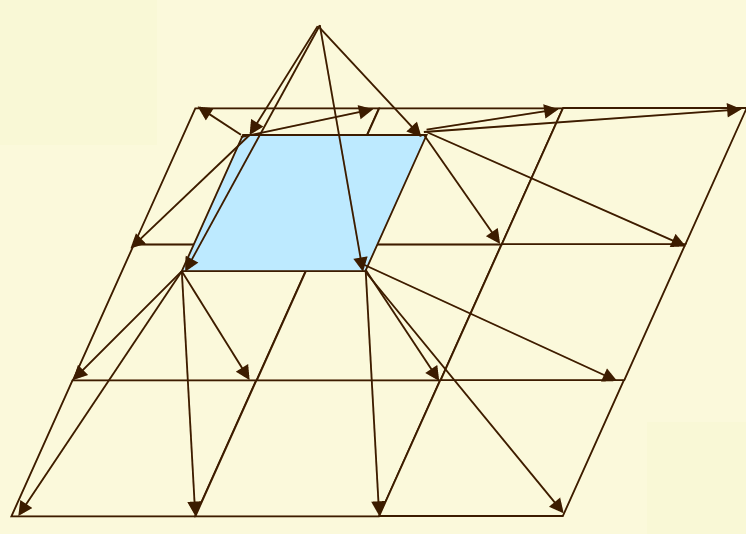
\includegraphics[width=0.5\linewidth]{figures/screenshot096}
\caption{Pyramid connectivity scheme.}
\label{fig:screenshot096}
\end{figure}

\item \textbf{Hypercube}: Consists of $2^N$ processors, each of which has $N$ links; depicted in \autoref{fig:screenshot097}. It is fault tolerant, and has shorter pathways than a mesh arrangement.

\begin{figure}
\centering
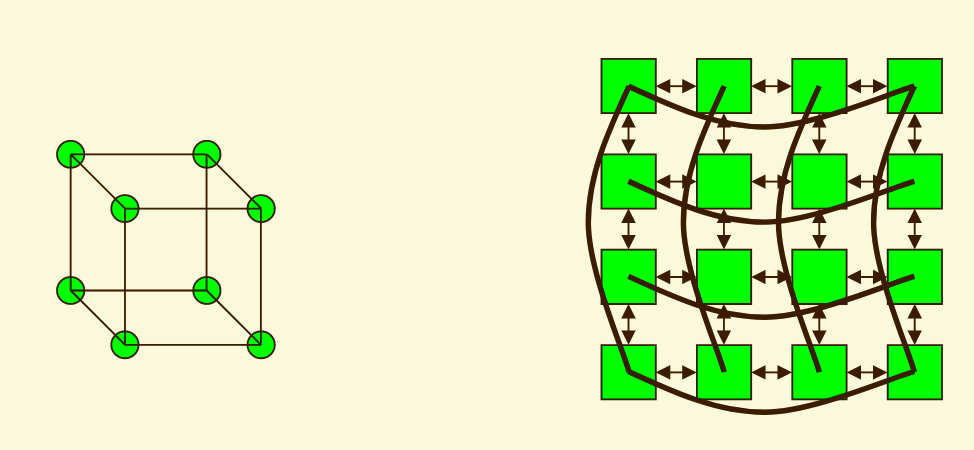
\includegraphics[width=0.5\linewidth]{figures/screenshot097}
\caption{Hypercube connectivity scheme.}
\label{fig:screenshot097}
\end{figure}

\item \textbf{Multistage} 
\item \textbf{Reconfigurable} 
\item \textbf{Crossbar} 
\item \textbf{Bus}
\end{itemize}

\section{Architectures}
There are four primary classes of data parallel architectures: SIMD (\autoref{fig:screenshot098}), systolic/pipelined (\autoref{fig:screenshot099}), vectorising (\autoref{fig:screenshot100}), and associative/neural (\autoref{fig:screenshot101}). These are compared in \autoref{tab:dataparallelsystems}.
\begin{table}[H]
\caption{A comparison of the principal characteristics of data-parallel systems.}
\label{tab:dataparallelsystems}
\begin{tabular}{|c|c|c|c|c|c|c|}
\hline 
\textbf{Property} & \textbf{SIMD} & \textbf{Systolic} & \textbf{Pipeline} & \textbf{Vectorizing} & \textbf{Neural} & \textbf{Associative} \\ 
\hline 
\textbf{Programmability} & Good & Fixed & Fixed & Good & Poor & Good \\ 
\hline 
\textbf{Availability} & Good & Poor & Poor & Good & Poor & Poor \\ 
\hline 
\textbf{Scalability} & Good & Fixed & Fixed & Fixed & Fixed & Good \\ 
\hline 
\textbf{Applicability} & Wide & Narrow & Narrow & Wide & Narrow & Wide \\ 
\hline 
\end{tabular} 
\end{table}

\begin{figure}
\centering
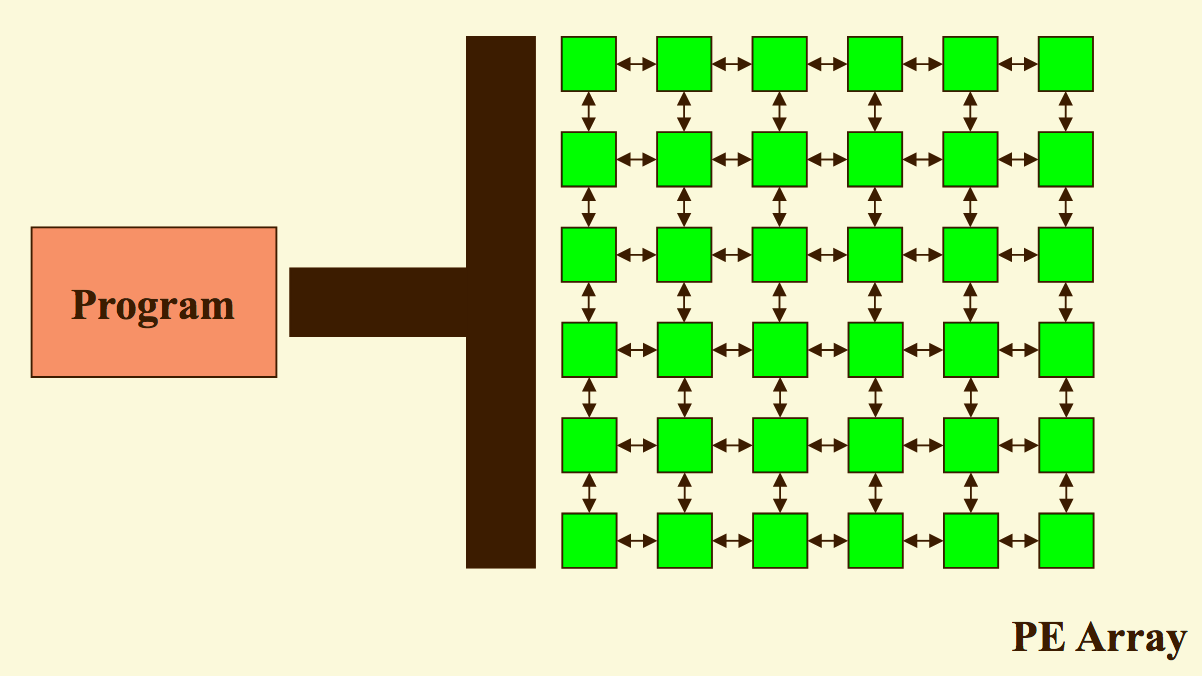
\includegraphics[width=0.5\linewidth]{figures/screenshot098}
\caption{SIMD data-parallel architecture.}
\label{fig:screenshot098}
\end{figure}

\begin{figure}
\centering
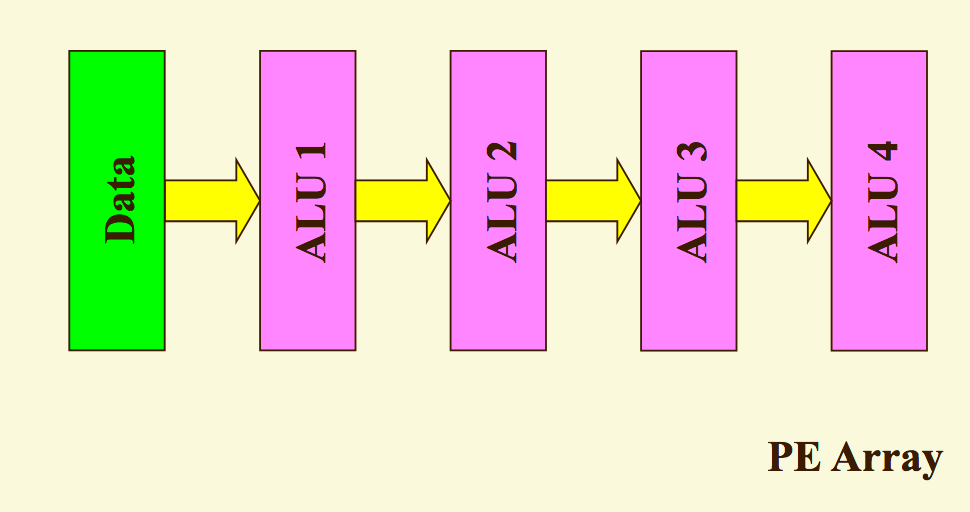
\includegraphics[width=0.5\linewidth]{figures/screenshot099}
\caption{Systolic/pipelined architecture.}
\label{fig:screenshot099}
\end{figure}

\begin{figure}
\centering
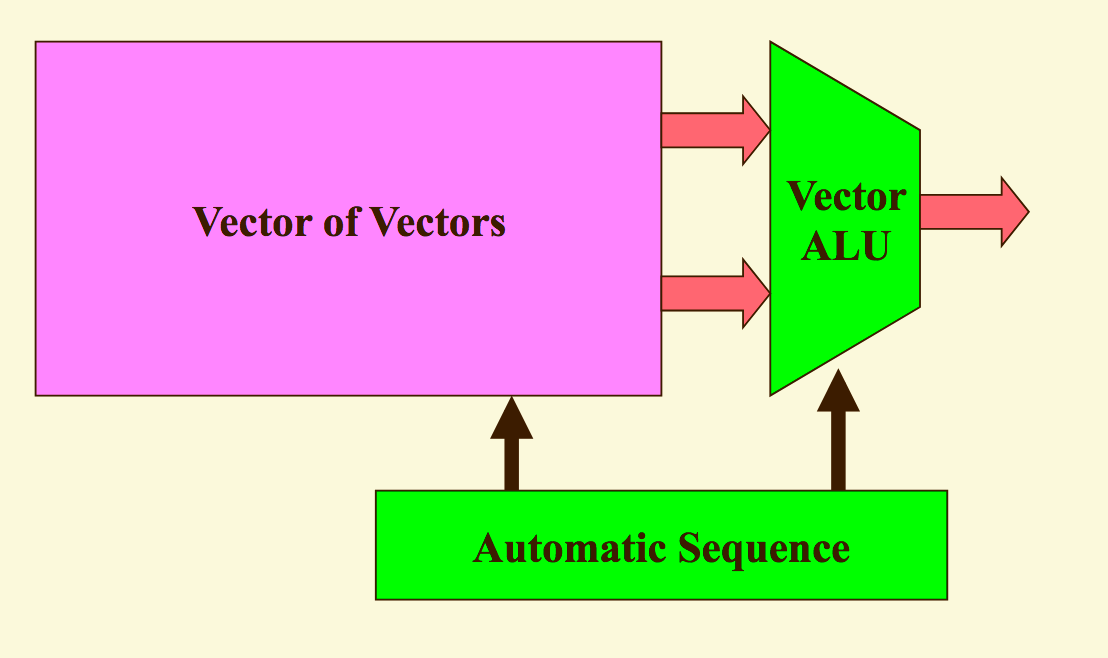
\includegraphics[width=0.5\linewidth]{figures/screenshot100}
\caption{Vectorising architecture.}
\label{fig:screenshot100}
\end{figure}

\begin{figure}
\centering
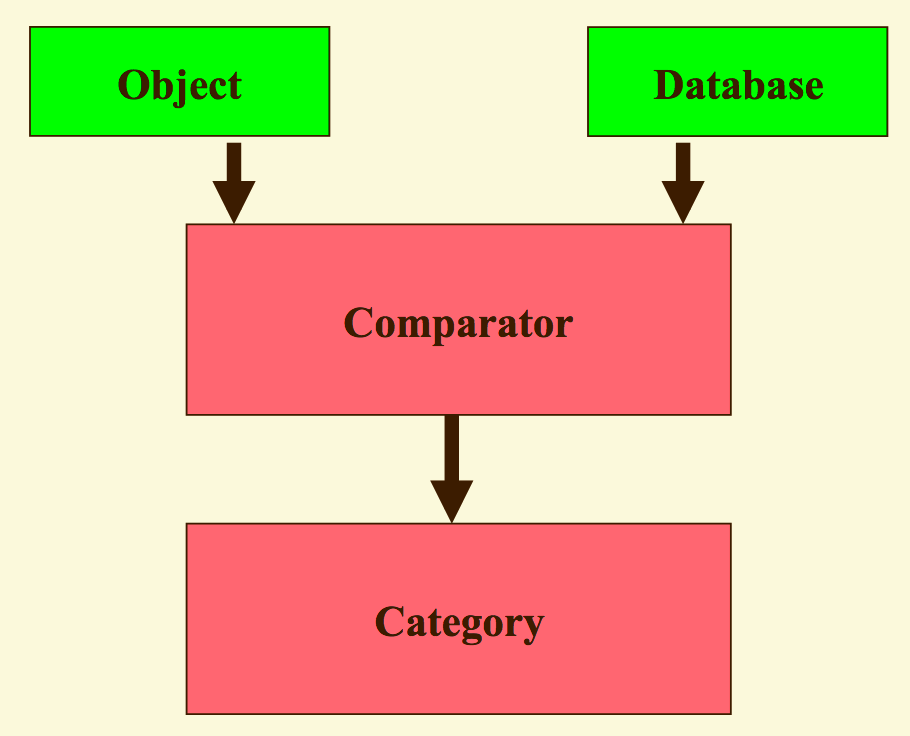
\includegraphics[width=0.5\linewidth]{figures/screenshot101}
\caption{Associative/neural architecture.}
\label{fig:screenshot101}
\end{figure}

\section{SIMD}
SIMD systems offer simplicity of programming, regularity of structure, scalability (both in size and performance), and wide applicability. The archetypal SIMD system is depicted in \autoref{fig:screenshot102}. The basic ideas, as formulated in 1958, are as follows: \begin{itemize}
\item Two dimensional array of processing elements 
\item All processors execute the same instruction simultaneously 
\item Each processor incorporates local memory 
\item Processors are programmable 
\item Data can propagate through the array 
\end{itemize}

\begin{figure}
\centering
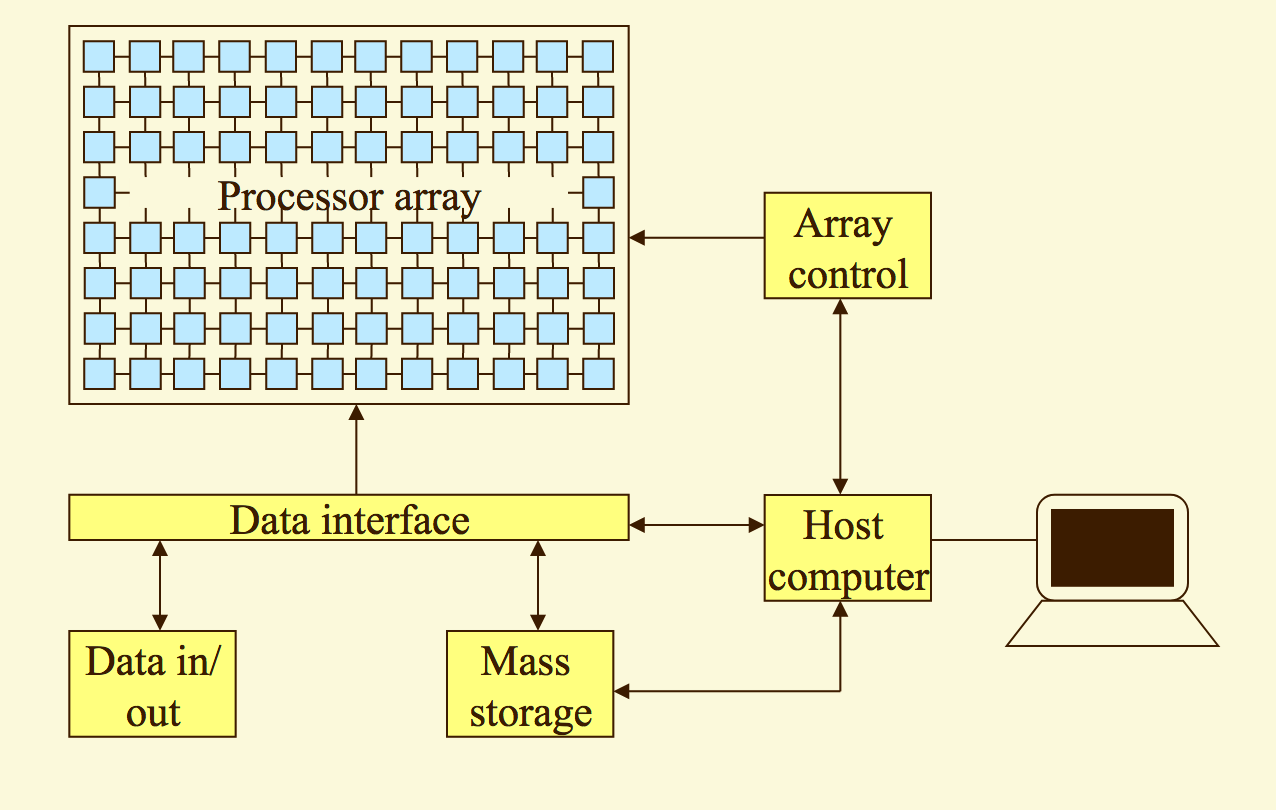
\includegraphics[width=0.7\linewidth]{figures/screenshot102}
\caption{The archetypal SIMD system.}
\label{fig:screenshot102}
\end{figure}

When designing a SIMD system to solve a problem, it is important to consider granularity. Fine-grained systems attempt to map one data element to one PE as closely as possible, while coarse-grained systems relax this and allow one PE to handle multiple data elements. This is depicted in \autoref{fig:screenshot103}.

\begin{figure}
\centering
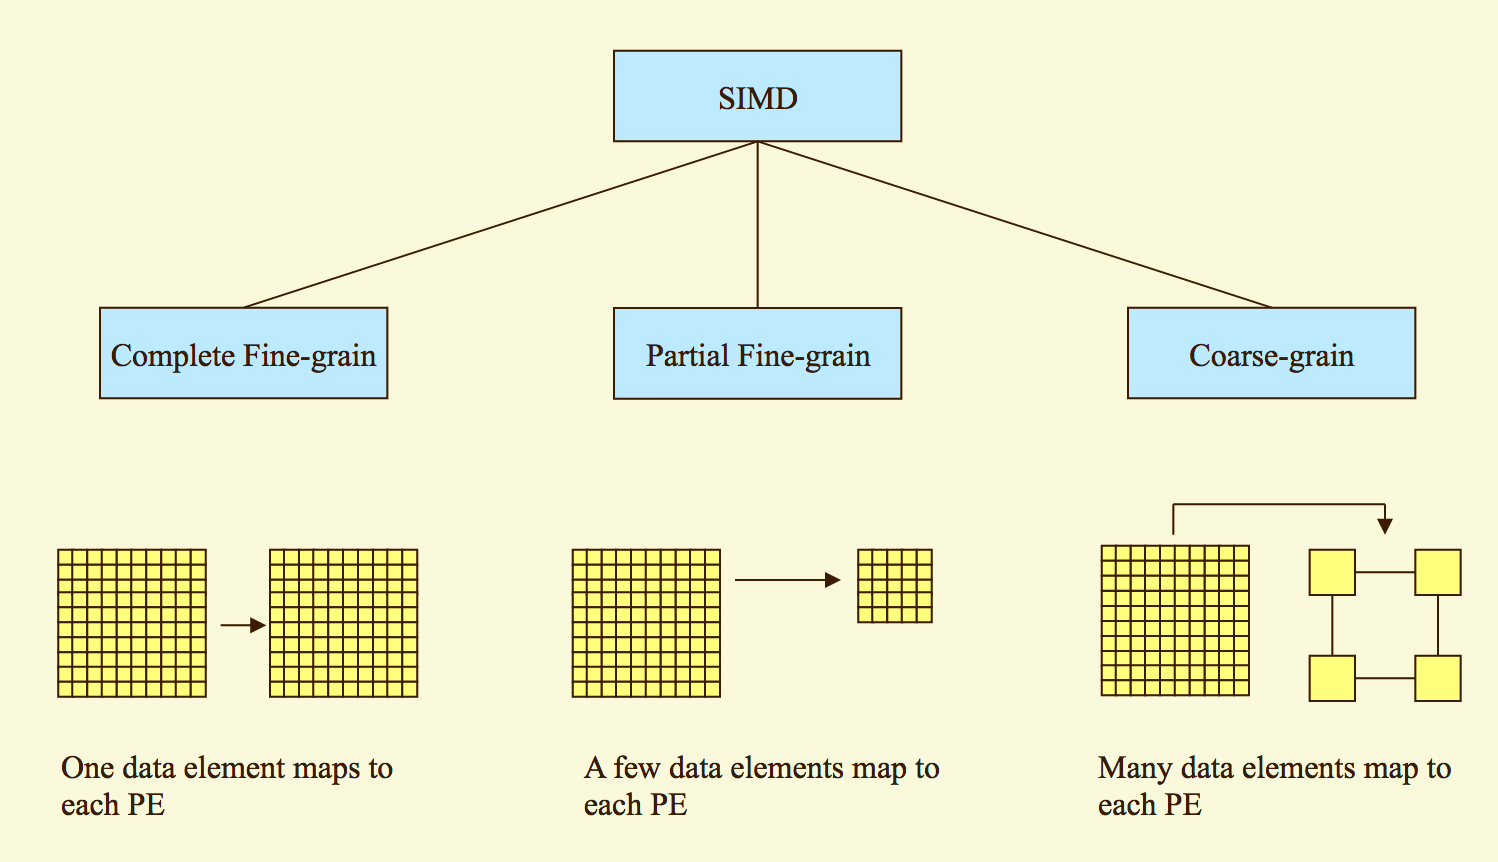
\includegraphics[width=0.7\linewidth]{figures/screenshot103}
\caption{Design space for granularity in a SIMD system.}
\label{fig:screenshot103}
\end{figure}

Additionally, the connectivity of the system should be explored, as discussed in \autoref{sec:connectivity}. Potential choices are depicted in \autoref{fig:screenshot104}.

\begin{figure}
\centering
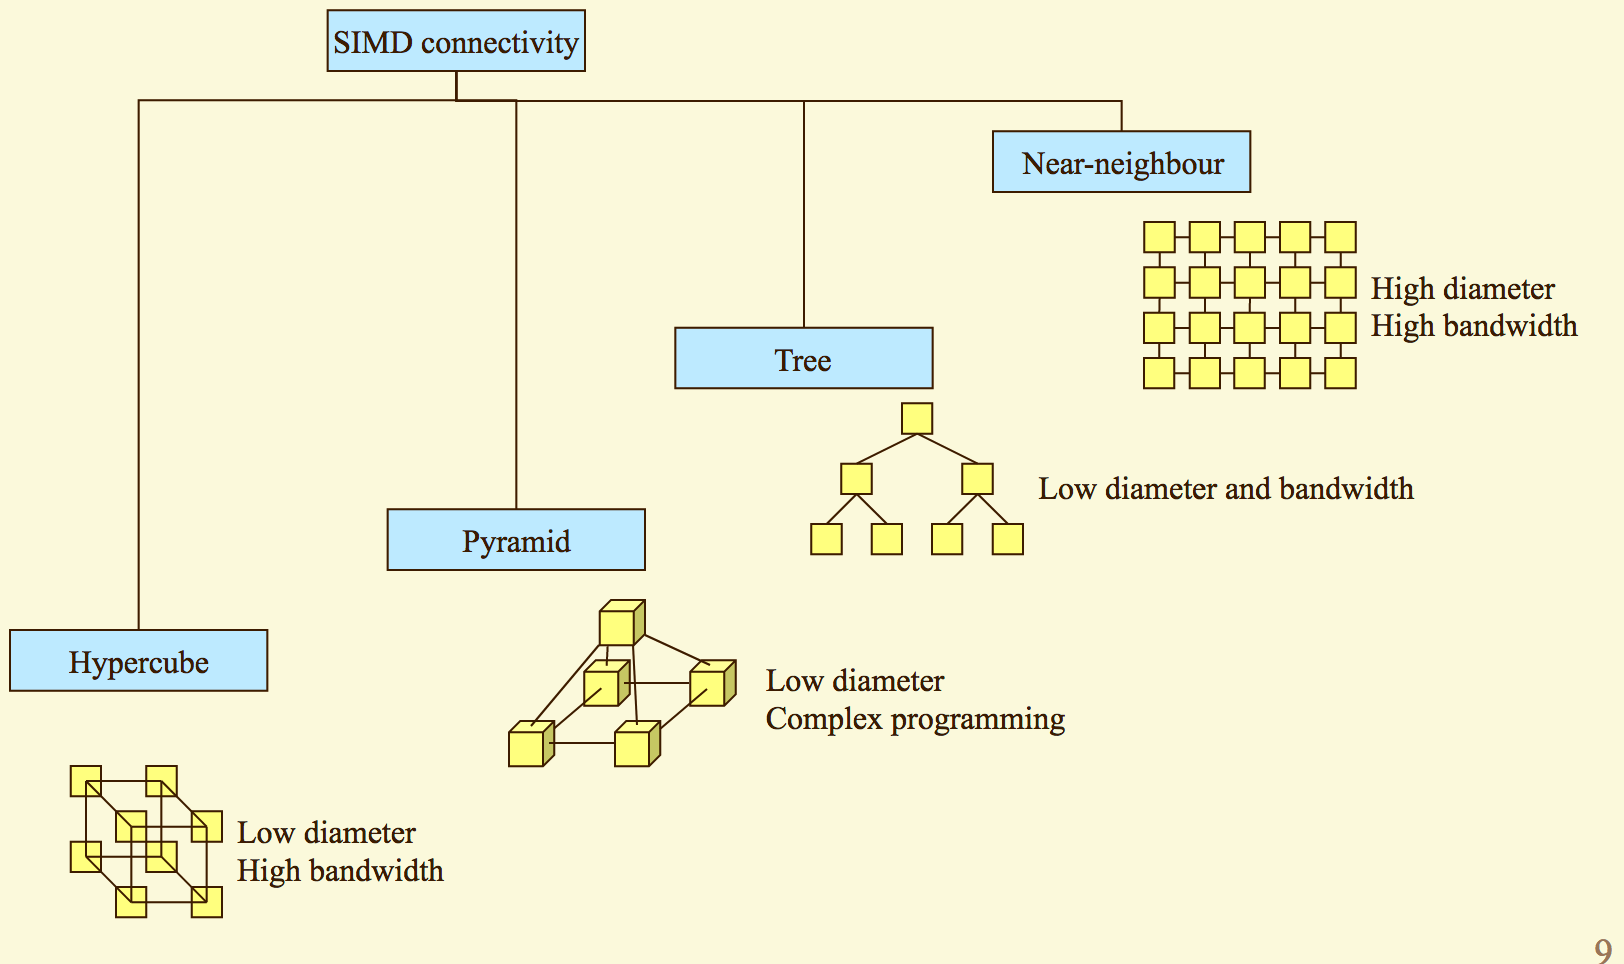
\includegraphics[width=0.7\linewidth]{figures/screenshot104}
\caption{Design space for SIMD connectivity.}
\label{fig:screenshot104}
\end{figure}

The granularity of the system also applies to the data type used for individual data elements, as shown in \autoref{fig:screenshot105}. PEs may also have a degree of local autonomy, as explored in \autoref{fig:screenshot106}.

\begin{figure}
\centering
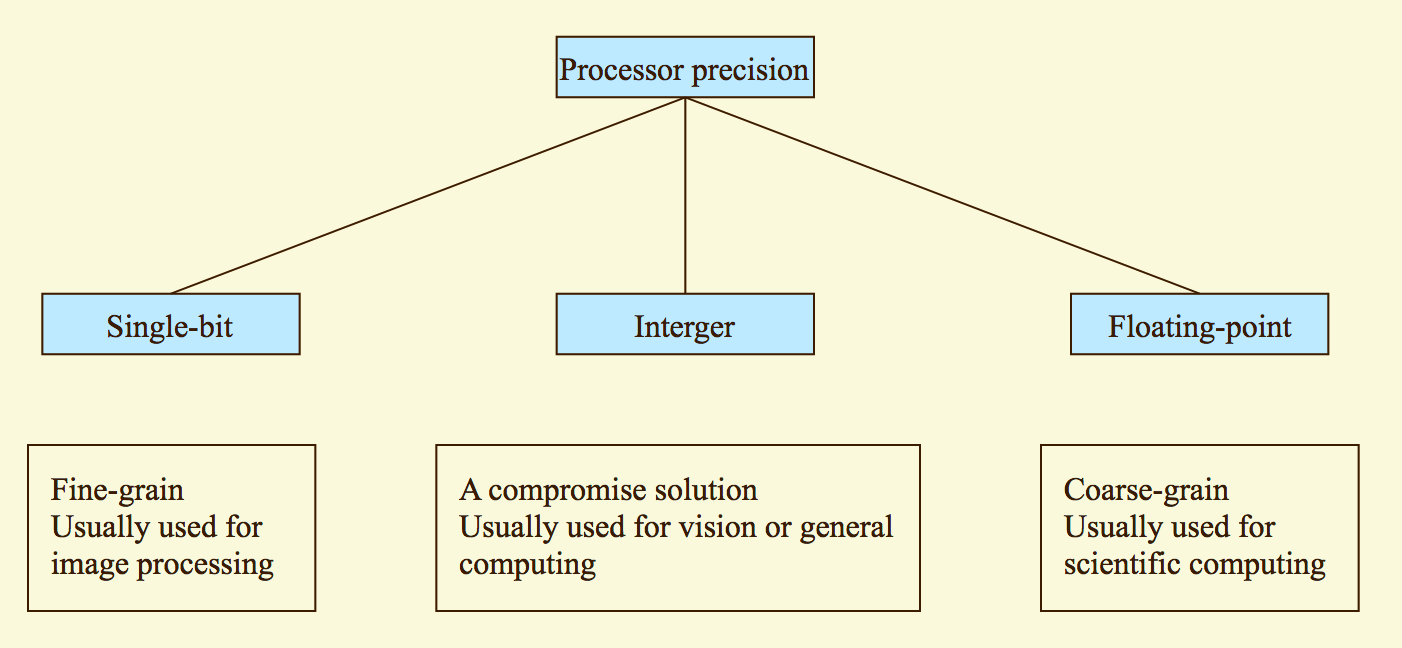
\includegraphics[width=0.7\linewidth]{figures/screenshot105}
\caption{Design space for processor complexity in a SIMD system.}
\label{fig:screenshot105}
\end{figure}

\begin{figure}
\centering
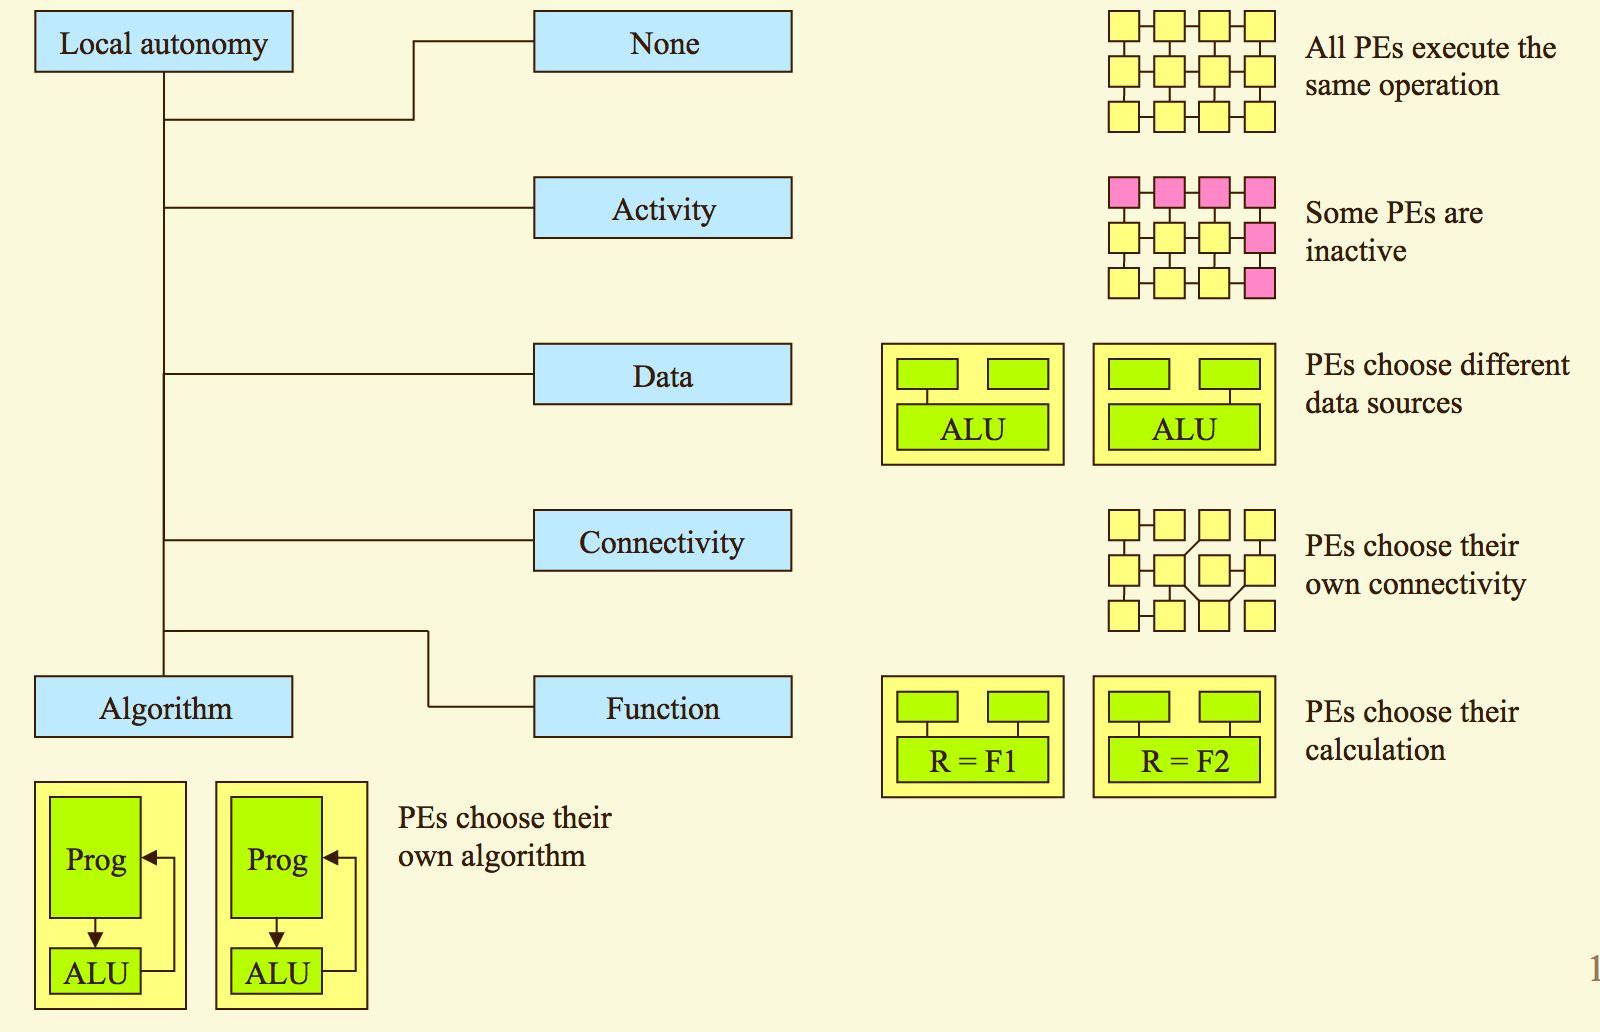
\includegraphics[width=0.7\linewidth]{figures/screenshot106}
\caption{Design space for local autonomy.}
\label{fig:screenshot106}
\end{figure}

\subsection{Example}
The SIMD architecture can be illustrated using the ILLIAC IV computer, which has only one control unit and 64 processing elements (\autoref{fig:screenshot107}). Each processing element has a 2K word memory attached. Each processing element performs the same operation, but they may be active or inactive. 

If they are inactive then they ignore the instruction. In this way the instruction may be applied to certain data elements and not others. For example, there is an instruction which disables all PE's active status if their accumulator is greater than 0.

Each processing element can transfer data to 4 other processing elements using a routing network; each element is also a full ALU capable of executing a wide range of arithmetic and logic functions. 

Each element has 6 registers: \begin{itemize}
\item \textbf{A}: accumulator 
\item \textbf{B}: second operand  
\item \textbf{R}: routing register 
\item \textbf{S}: temporary storage 
\item \textbf{X}: index register 
\item \textbf{D}: mode register (active/inactive) 
\end{itemize}

\begin{figure}
\centering
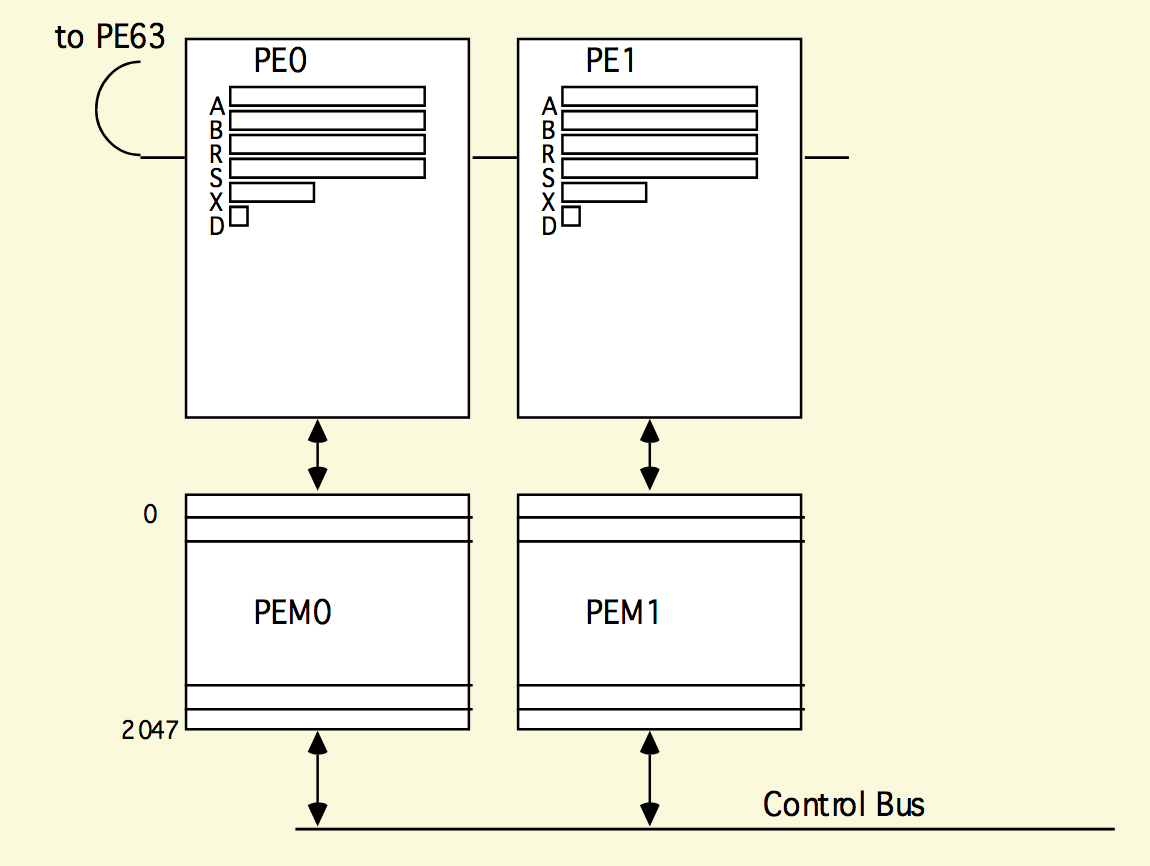
\includegraphics[width=0.7\linewidth]{figures/screenshot107}
\caption{ILLIAC IV machine structure.}
\label{fig:screenshot107}
\end{figure}

Each PEM contains 2048 64 bit words of data. PEMi can only be addressed from PEi. Thus a PE can only change data in its own PEM. Data can be passed from PE to PE via the routing network, shown in \autoref{fig:screenshot108}. The control unit bus allows instructions to be fetched from PEMs. Data can be broadcast to all PEs using a broadcast bus. Data is passed between processing elements using the routing network. 

\begin{figure}
\centering
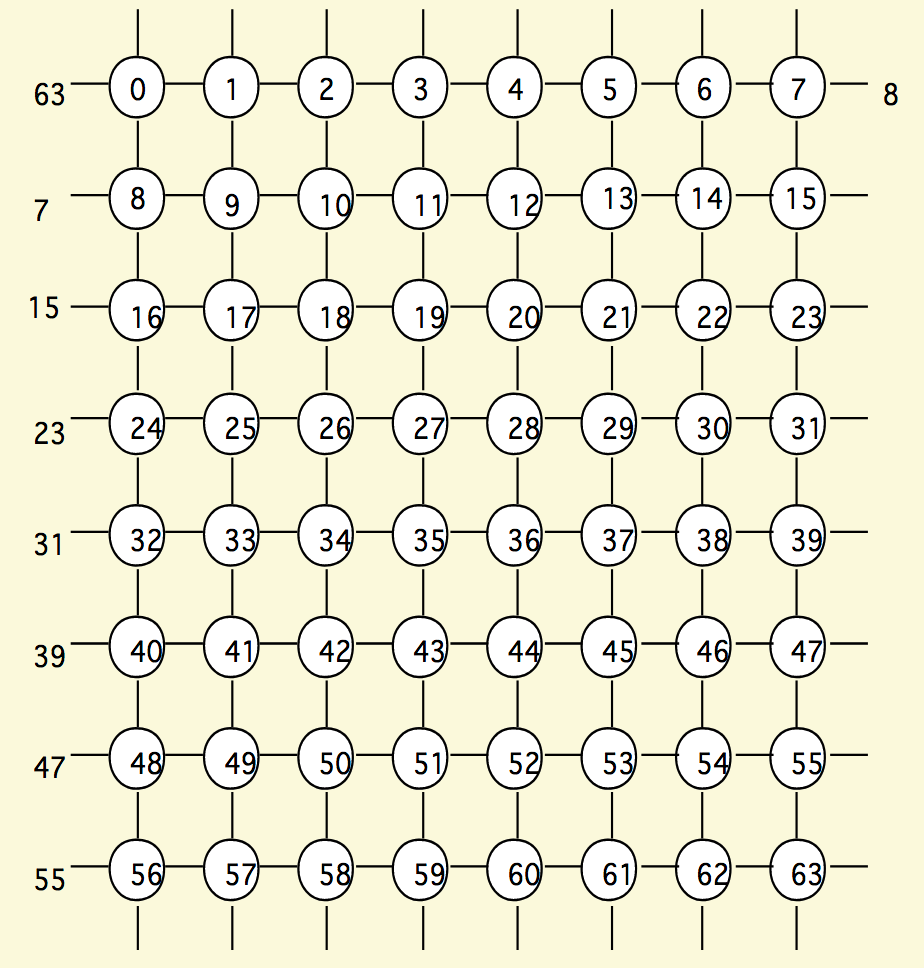
\includegraphics[width=0.7\linewidth]{figures/screenshot108}
\caption{ILLIAC IV connectivity.}
\label{fig:screenshot108}
\end{figure}

Array addition $A(i) = B(i) + C(i)$ for $1 < i \le N = 64$ can be handled in a vectorised fashion, offering a speedup of $N$ times. The instruction stream is simple: load from location 2, add to location 1, store in location 0. If $N < 64$, then some of the processing elements must be disabled. If $N > 64$, the code must loop until $N$ is exhausted.

Consider $A(i) = B(i) + A(i-1)$ for $2 < i \le 64$. This is a serial loop, and therefore cannot be run concurrently. Expanding out the loop gives: \begin{itemize}
\item $A(2) = B(2) + A(1)$
\item $A(3) = B(3) + A(2)$
\item $\dots$
\item $A(64) = B(64) + A(63)$
\end{itemize}
However, this is a recurrence relationship, so it can be rewritten as such:
\begin{itemize}
\item $A(2) = B(2) + A(1)$
\item $A(3) = B(3) + B(2) + A(1)$
\item $A(4) = B(4) + B(3) + B(2) + A(1)$
\item $\dots$
\end{itemize}
This rearrangement allows calculation of $A$ independently from the loop:
\begin{algorithmic}
\State $S \gets A(1)$
\For{N = 2, 64}
	\State $S \gets S + B(N)$
\EndFor
\State $A(N) = S$
\end{algorithmic}
This reformulation is still a sequential algorithm, however. \textit{Recursive doubling} can be used to execute in log time, as shown in \autoref{fig:screenshot109}.

\begin{figure}
\centering
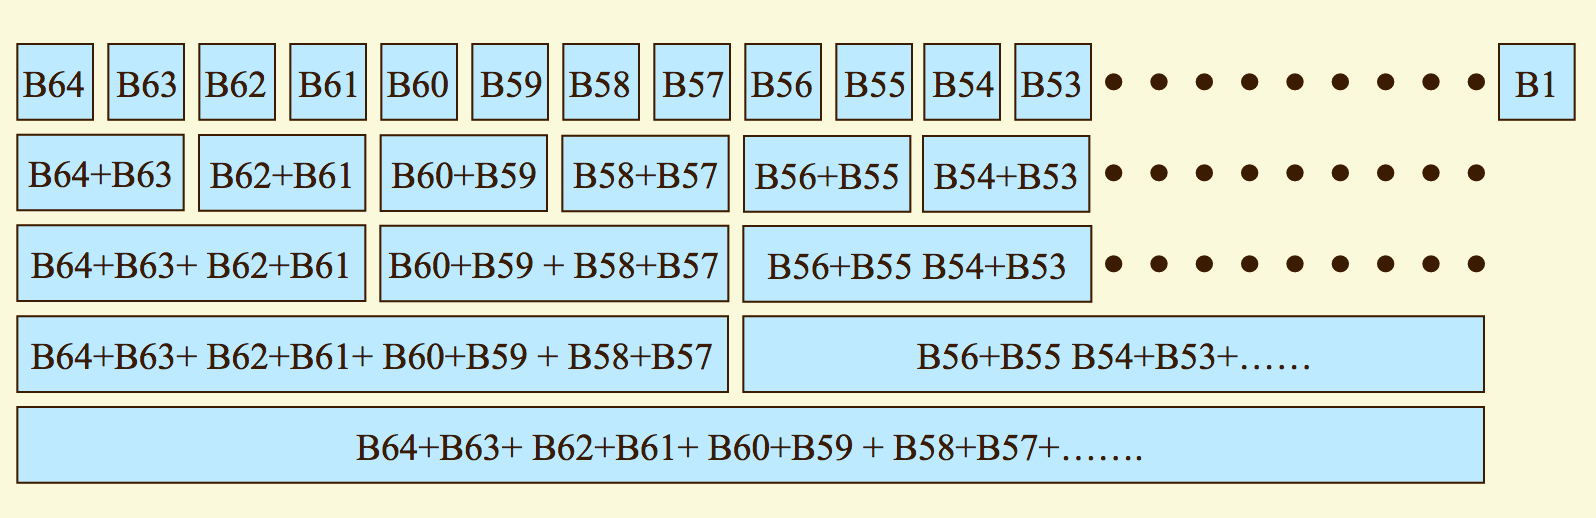
\includegraphics[width=0.7\linewidth]{figures/screenshot109}
\caption{Recursive doubling algorithm.}
\label{fig:screenshot109}
\end{figure}

This algorithm is shown below \footnote{I made the executive decision to not rewrite any algorithms longer than 6 lines. Maybe for version 2!}:
\begin{lstlisting}[language={}]
1. Enable all PE's (Turn on all PE's) 
2. All PE's load RGA from location B 
3. i = 0 
4. All PEs load RGR from their RGA 
5. All PEs ROUTE their RGR contents 2i to the right. 
6. j = 2i -1 
7. Disable all PE's number 0 through j 
8. All enabled PE's ADD RGA to RGR 
9. i = i + 1 
10. if i < 6 goto 4 
11. Enable all PEs 
12. All PEs store RGA to A 
\end{lstlisting}
